\setchapterpreamble[u]{\margintoc}
\chapter{Frattura}
\labch{cap10}

Un materiale metallico deve essere \textbf{resistente}, cioè avere un elevato carico di rottura (anche elevato carico di snervamento) che viene misurato tramite prova di trazione, e \textbf{tenace}, cioè deve possedere un elevata energia di rottura misurata tramite prova di resilienza. La frattura dipende dal tipo di materiale e dal tipo di sollecitazione: quella triassiale si usa per i materiali fragili, quella monoassiale per i materiali tenaci.\\
Il vetro, ad esempio, è resistente, ma non tenace.\\
La frattura può essere suddivisa in duttile e fragile, a sua volta divisibile in intergranulare ed intragranulare.

Nel caso di \textbf{frattura duttile} su \textbf{monocristalli}, dove in questo caso si attiva un solo piano di scorrimento in una sola direzione senza incrudimento. Sappiamo che lo sforzo di taglio è massimo se ha un inclinazione di 45°: si ottiene quindi la frattura plastica su un piano a 45°. Se invece si attivano più piani di scorrimento si può arrivare ad avere la sezione finale che può ridursi in un punto. E’ il caso di una lamiera, ma è raro.\\
Nel caso di \textbf{frattura duttile} su \textbf{policristalli}, la frattura inizia al centro del provino, in un piano macroscopicamente perpendicolare all’asse del carico applicato, a causa della presenza di inclusioni. Il materiali intorno all’inclusione si distacca e si crea una fessura. All’apice di questa fessura il carico tensionale è massimo e si formano delle bande di taglio a 45° . La fessura originale comincia a deviare a questa inclinazione, fino a quando la fessura si inclina nuovamente (si va avanti a zig-zag).Questo processo va avanti fino a quando la fessura interessa l’intera sezione resistente giungendo a rottura, denominata \textbf{frattura coppa e cono}, e il materiale si strappa.\\
La fessura centrale si forma per nucleazione e crescita di cavità interne dovute all’interazione di dislocazioni ed inclusioni. Infatti, l’aumento di dislocazione causa il distacco fra particella e matrice. Per nucleare una struttura occorre che ci si una certa deformazione critica:
\begin{equation*}
    \varepsilon=\sqrt{\frac{\gamma}{4\mathrm{GR}}}
\end{equation*}

dove R è il raggio delle particelle e $\gamma$ è l’energia superficiale.\\
La tensione critica per la nucleazione di una cavità vale:
\begin{equation*}
    \sigma=\sigma_0 + (\mathrm{cG\gamma})^{1/2}\Bigg(\frac{f^{2/3}}{\mathrm{R}}\Bigg)^{1/2}
\end{equation*}
dove c e $\sigma_0$ sono delle costanti ed f indica la frazione volumetrica.\\
Dopo che è avvenuta nucleazione, vi è la crescita, che consiste nell’allungamento della frattura.

I parametri che influiscono sulla duttilità sono:
\begin{itemize}
    \item frazione volumetrica totale di particelle di seconde fasi (purezza del materiale);
    \item natura delle particelle: legate più o meno fortemente alla matrice;
    \item dimensioni delle particelle: più le particelle sono piccole maggiore deve essere l’energia di nucleazione;
    \item forma delle particelle (fenomeno del traverso);
    \item resistenza della matrice: più la matrice è tende più il materiale avrà un comportamento duttile;
    \item presenza di idrogeno;
    \item capacità di incrudimento e dimensioni dei piani della matrice: c’è bisogno di avere un elevato coefficiente di incrudimento, affinché aumenti il carico di rottura. La sollecitazione, così, si distribuisce e non si arriva alla rottura.
\end{itemize}

Nel caso di \textbf{frattura fragile}, detta anche \textbf{sfaldatura}, non vi è deformazione plastica. E’ favorita dalle temperature basse ed è caratterizzata dallo scarso assorbimento di energia. Tale tipologia di frattura è nociva e molto pericolosa perché la fessura si espande ad alta velocità. Questo tipo di frattura non è osservabile nei reticolo CFC, perché sono presenti molti piani di scorrimento, quindi ce ne sarà sempre qualcuno attivo: questo è il grande vantaggio degli acciai austenitici. Focalizzandosi sul carico teorico di frattura, si osserva che esso comporta la rottura dei legami e la creazione di nuove superficie. L’energia deriva dall’energia di deformazione plastica. Si può dimostrare che:
\begin{equation*}
    \sigma_t = \sqrt{\frac{\gamma E}{a}}
\end{equation*}\sidenote{a è la costante reticolare.}
Prendendo ad esempio come riferimento una lastra piana contenente una fessura ellittica lunga 2c con $\rho$ raggio di curvatura all’estremità dell’ellisse:
\begin{equation*}
    \sigma_{estremita'} = 2\sigma\sqrt{\frac{\mathrm{c}}{\rho}}
\end{equation*}
La frattura avviene quando:
\begin{equation*}
    2\sigma\sqrt{\frac{\mathrm{c}}{\rho}} = \sqrt{\frac{\gamma \mathrm{E}}{\mathrm{a}}}
\end{equation*}
da cui:
\begin{equation*}
    \boldsymbol{\sigma_{rottura} = \sqrt{\frac{\gamma \mathrm{E} \rho}{\mathrm{4ca}}}}
\end{equation*}

Quindi, raggi di curvatura piccoli, cioè presenza di intagli acuti, spigoli, favoriscono la frattura e la propagazione si autoalimenta, in quanto aumentando la lunghezza della cricca diminuisce la tensione necessaria affinché essa si propaghi.\\
Le fessure si creano se si hanno ostacoli nel piano di scorrimento delle dislocazioni, oppure quando esse si intersecano. Durante la propagazione della fessura, l’energia di deformazione si trasforma in energia cinetica, superficiale e di deformazione plastica. Quest’ultimo termine dipende dal fatto che davanti alla fessura si ha una fortissima tensione a trazione localmente scomponibile in carichi di taglio su piani a 45°. I carichi di taglio di taglio nucleano dislocazioni su piani di scorrimento favorevolmente orientati.\\
La nucleazione è ridotta e quindi il termine di deformazione plastica risulta essere poco influente se vi sono basse temperature e/o velocità di incremento del carico elevata. La presenza di deformazione plastica ostacola la propagazione della fessura in quanto si ha uno scorrimento con assorbimento di energia per la nucleazione ed il movimento delle dislocazioni. Se il lavoro di deformazione plastica è elevato, la fessura può essere rallentata e fermata, grazie ai processi di platicizzazione. Infatti, i materiali CFC non danno sfaldatura perché hanno molti sistemi di scorrimento equivalenti, che si deformano plasticamente sottraendo energia alla propagazione della cricca. Le dislocazioni, inoltre, assorbono energia dalle fessura in movimento poiché quando vi è un intersezione fessura-dislocazione si formano sulle fessure delle tacche che ne ostacolano il movimento.\\
Il principale ostacolo alla propagazione delle fessure è il bordo di grano.
Si può dimostrare che:
\begin{equation*}
    \mathrm{Reistenza\> alla\> frattura = \frac{f}{\sqrt{d_{grani}}}}
\end{equation*}

Se il \textbf{diametro medio dei grani} supera un certo valore critico, il carico necessario ad espandere la fessura diventa più piccolo di quello necessario per nucleare una fessura entro il cristallo. La prima fessura che si forma può provocare la rottura del campione. Si ha in questo caso la \textbf{frattura a nucleazione limitata}, cioè vi sono pochi grani. In questo caso, il carico di rottura, pari al carico di nucleazione, è uguale al carico di snervamento.\\
Se il valore di diametro non raggiunge il valore critico si avranno grani piccoli quando nasce una fessura essa viene bloccata dal grano e se ne devono creare delle altre aumentando il carico. Si ha in questo caso la \textbf{frattura a propagazione limitata}, cioè vi sono molti grani. In questo caso, il carico di rottura è maggiore del carico di snervamento e durante la fase plastica vi è la nascita di molte microfratture.\\
Quanto detto è riassumibile nel diagramma di Gilman:
\begin{figure}[hb]
    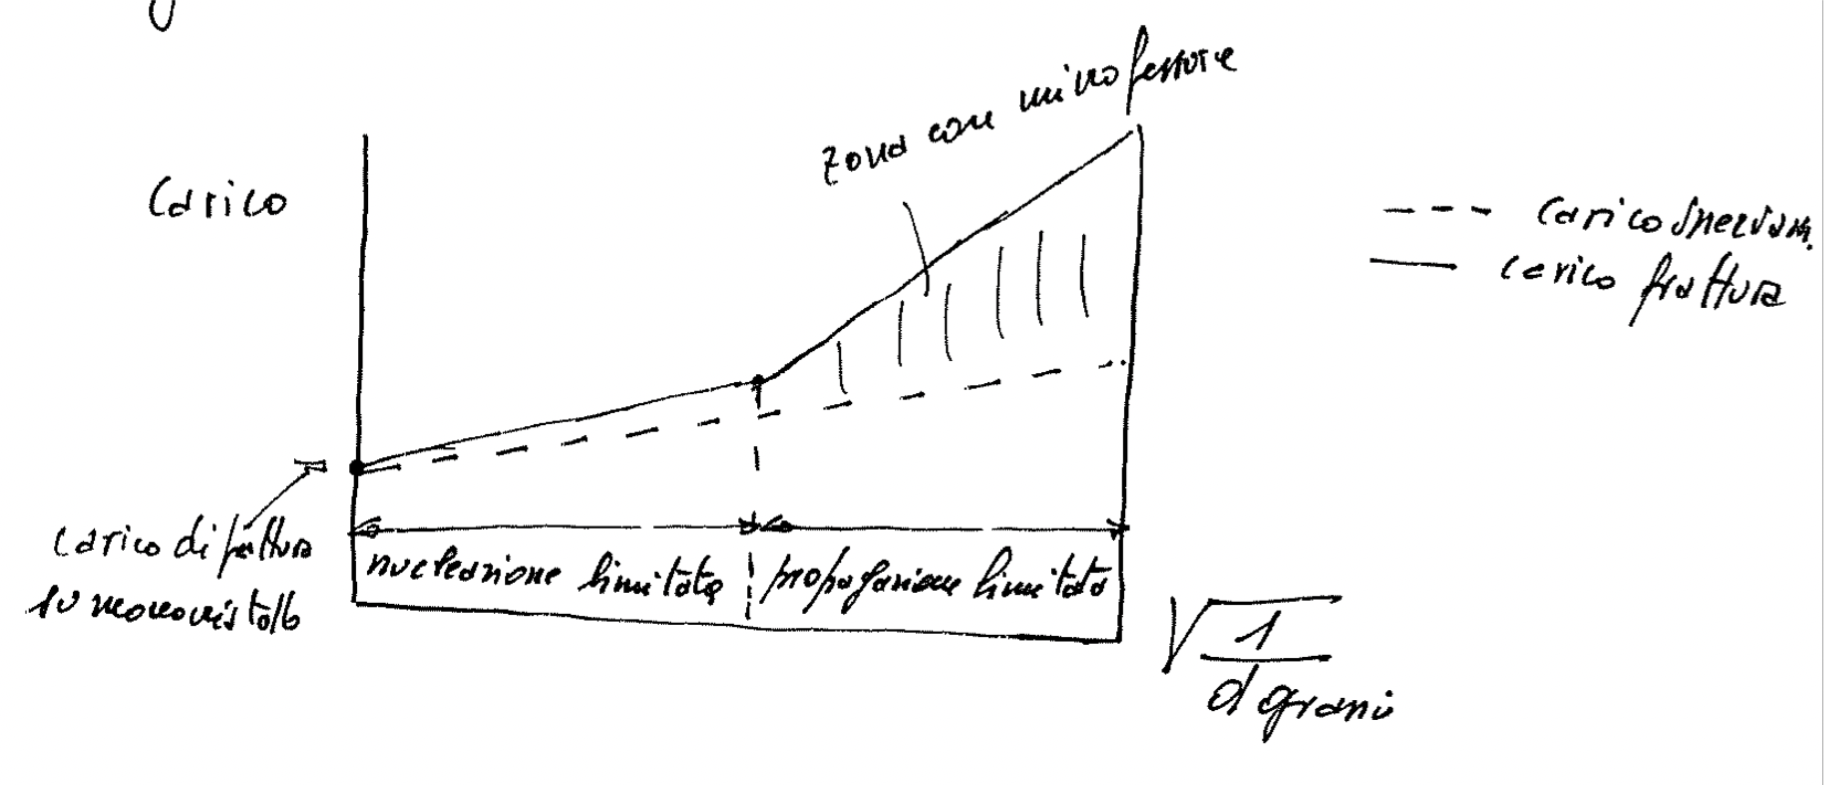
\includegraphics[width=0.8\textwidth]{images/img35.png}
    \caption{Diagramma di Gilman}
    \labfig{img35}
\end{figure}
La \textbf{sfaldatura} o \textbf{rottura fragile} è favorita da ogni sistema di carichi capace di produrre grandi carichi a trazione e piccoli carichi di taglio:
\begin{itemize}
    \item Se la tensione è uniassiale, il carico è equivalente a una serie di carichi di taglio a 45°;
    \item Se due carichi a trazione sono applicati a 90° l’uno dall’altro, le componenti di taglio sono opposti le une dalle altre. Se si applica un carico perpendicolare vi sarà uno stato di tensione idrostatica nel quale il materiale non subisce carico di taglio;
    \item Il carico più pericoloso che si può applicare è il carico triassiale perché favorisce la frattura fragile. Un carico triassale, oltre che ottenerlo dall’esterno, si può ottenere anche da un carico monoassiale se la sezione varia nel tempo.
\end{itemize}